% Compiler: LaTeX => PDF

\documentclass[xcolor=dvipsnames]{beamer}

\mode<presentation>
{
	\usetheme{BerlinHUB}
	%\setbeamercovered{transparent}
}

\usepackage[ngerman]{babel}
\usepackage[utf8]{inputenc}

\usepackage{helvet}
\usepackage[T1]{fontenc}

%\usepackage{multimedia}
%\usepackage{graphicx}
%\usepackage[nolist]{acronym}

%\usepackage{stackengine}
%\usepackage{array}

%\usepackage{enumitem}

%\setitemize{label=\usebeamerfont*{itemize item}%
%  \usebeamercolor[fg]{itemize item}
%  \usebeamertemplate{itemize item}}

\title[Streifenlichtprojektion]
{Streifenlichtprojektion und optische Analyse zur Oberflächeninspektion}

\author[D. Wagner, J. Spangenberg, L. Kramer]
{
	Dennis~Wagner
	\and
	Johannes~Spangenberg
	\and
	Leroy~Kramer
}

\institute[]
{
	Humboldt-Universität zu Berlin\\  
	Institut für Informatik\\
	Lehrstuhl Signalverarbeitung und Mustererkennung\\
	\vspace{1em}
	Semesterprojekt Signalverarbeitung\\
	bei Prof. Dr. Meffert
}

\date{12.02.2014}
\subject{Informatik}

% add logo of university
\pgfdeclareimage[height=0.75cm]{university-logo}{husiegel_bw_klein}
\logo{\pgfuseimage{university-logo}}


\begin{document}
\begin{frame}
	\titlepage
\end{frame}

\begin{frame}
	\frametitle{Gliederung}
	\tableofcontents
\end{frame} 

% ---------------------------------------------------------------------------- %

\section{Motivation} 
\begin{frame}
	\frametitle{Motivation}

	\begin{itemize}
		\item Günstige Messmethode
		\item Messung ohne Kontakt zum Objekt möglich
		\item Wird in vielen Bereichen verwendet:
		\begin{itemize}
			\item Computer Grafik
			\item Robotik
			\item Archäologie
			\item Geographie
			\item Reverse Engineering
			\item Computerunterstütze Qualitätskontrolle
			\item \dots
		\end{itemize}
	\end{itemize}

\end{frame}


\section{Unsere Aufgabe} 
\begin{frame}
	\frametitle{Unsere Aufgabe}

	\vfill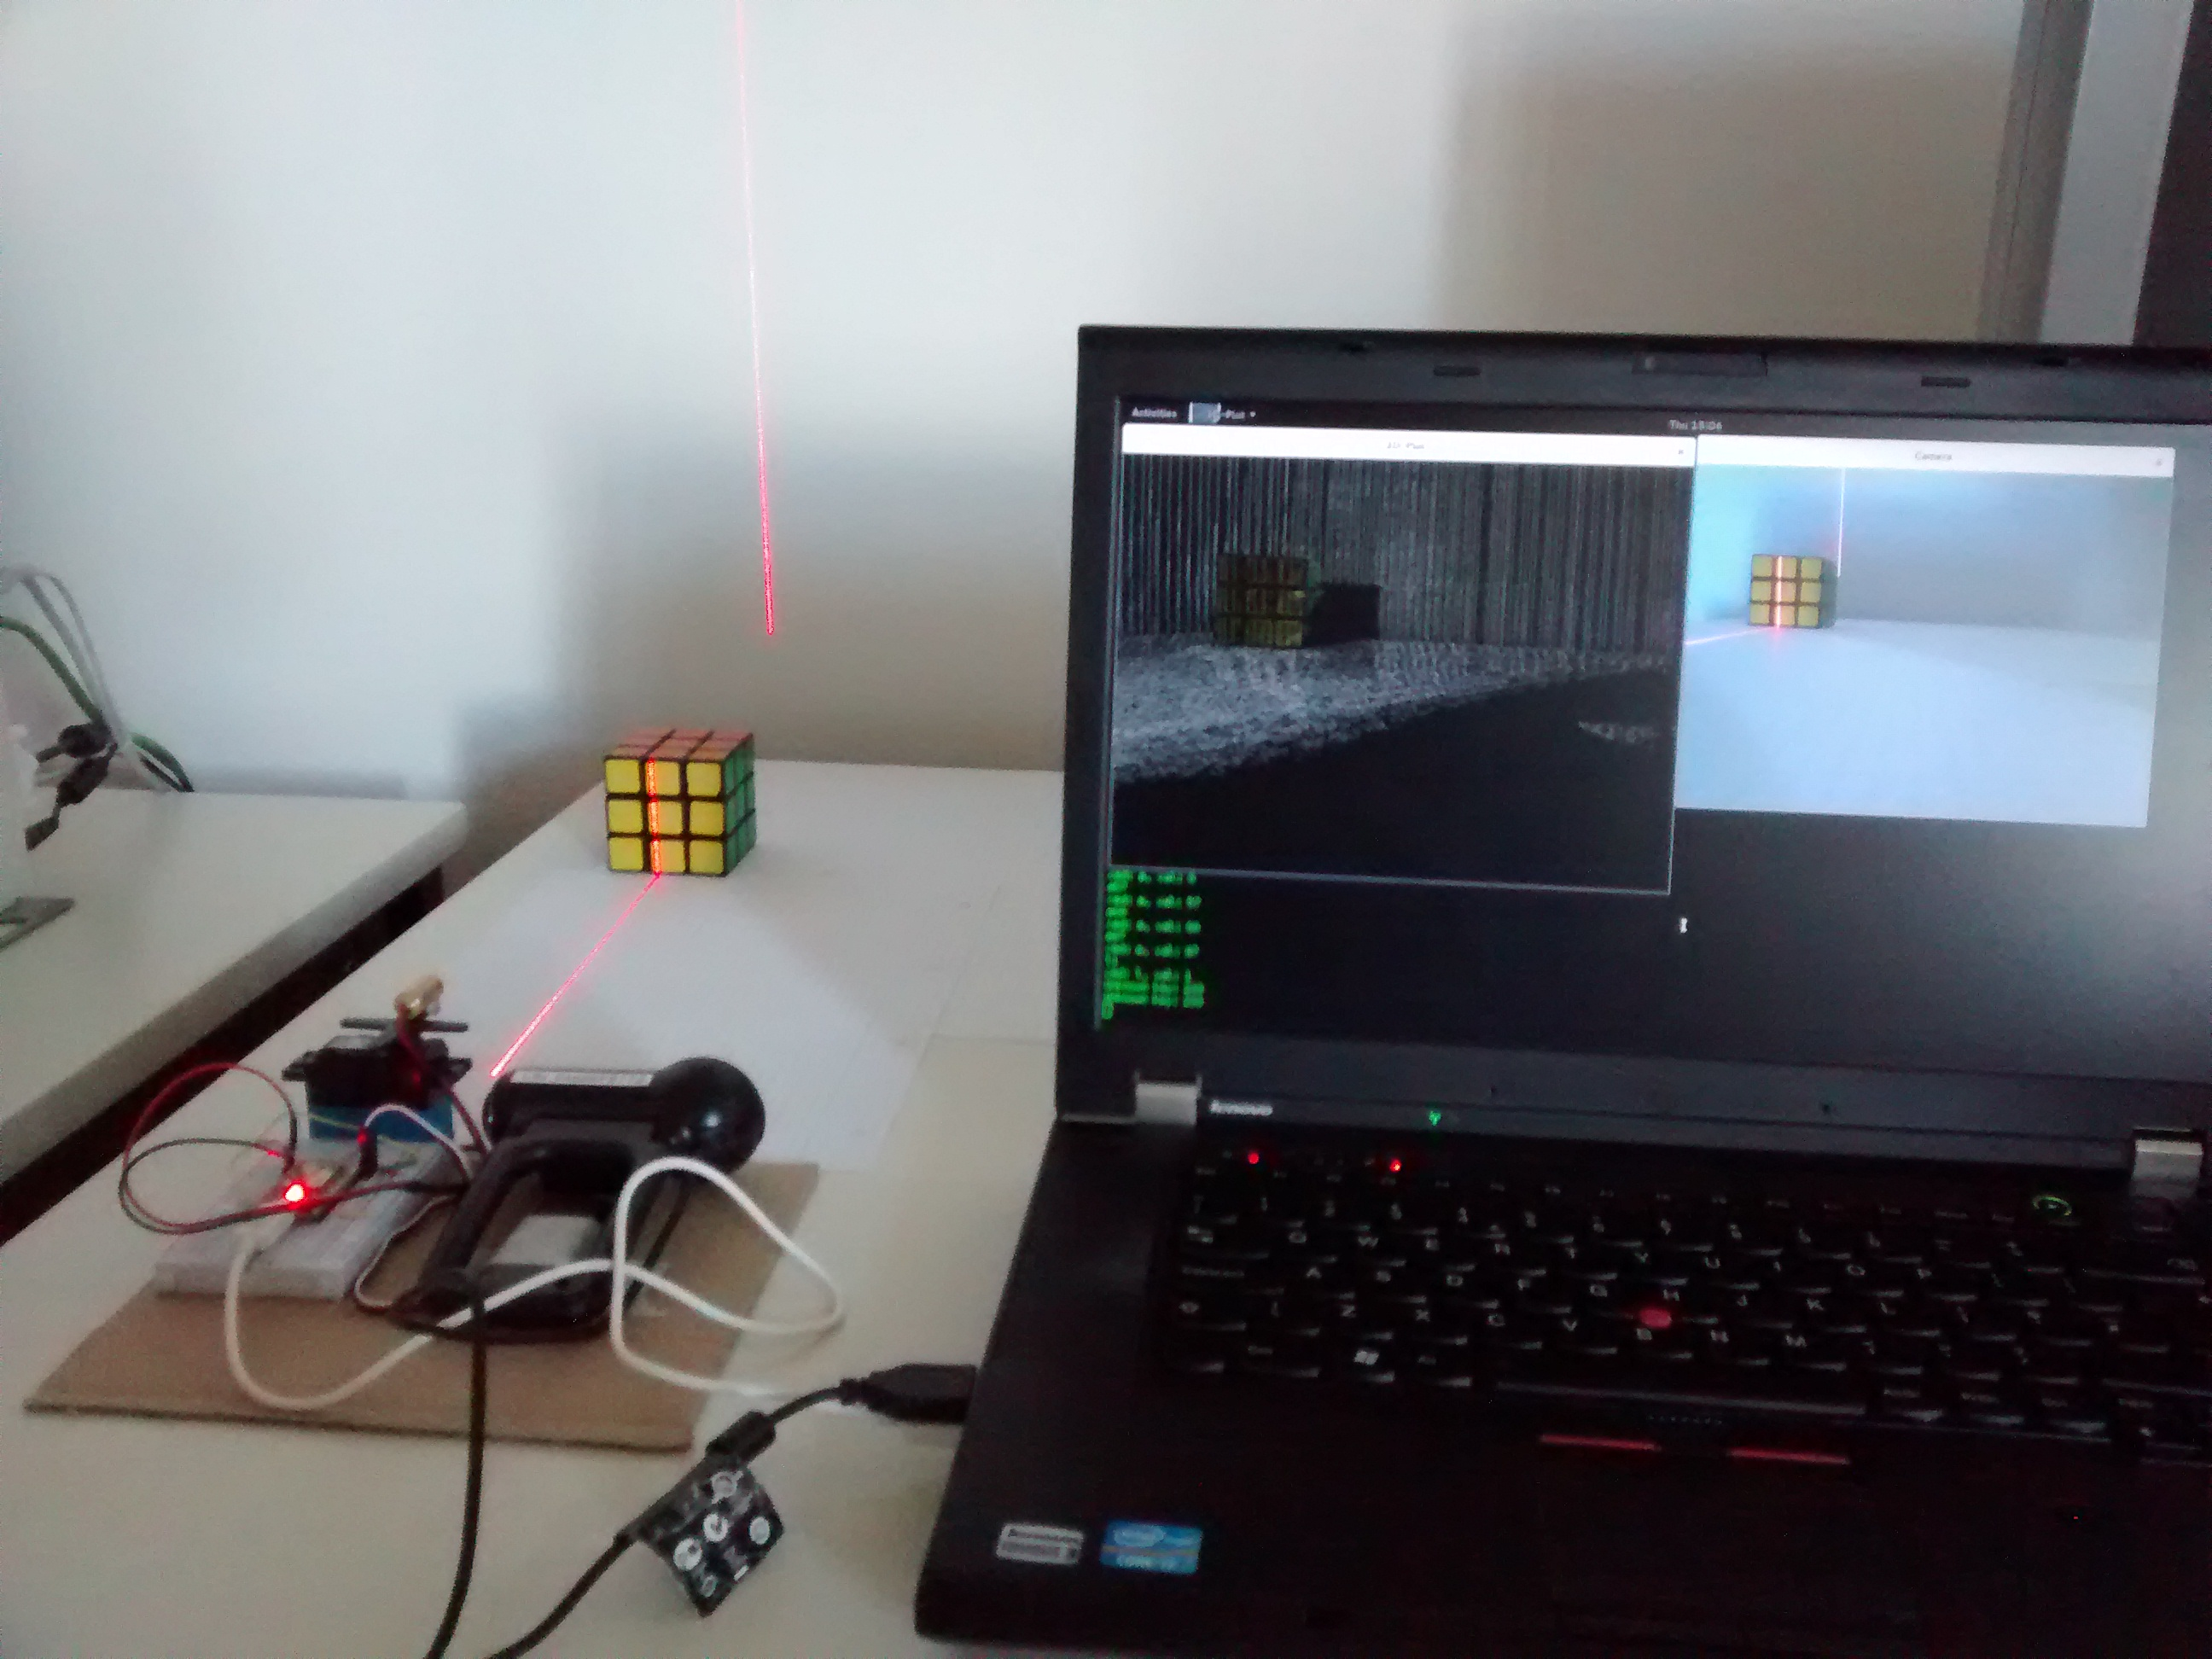
\includegraphics[width=\linewidth]{includes/setup}\vfill

\end{frame}

% ---------------------------------------------------------------------------- %

\section{Umsetzung} 
%\subsection{Hardware}
\begin{frame}
	\frametitle{Umsetzung}
	\framesubtitle{Hardware}

	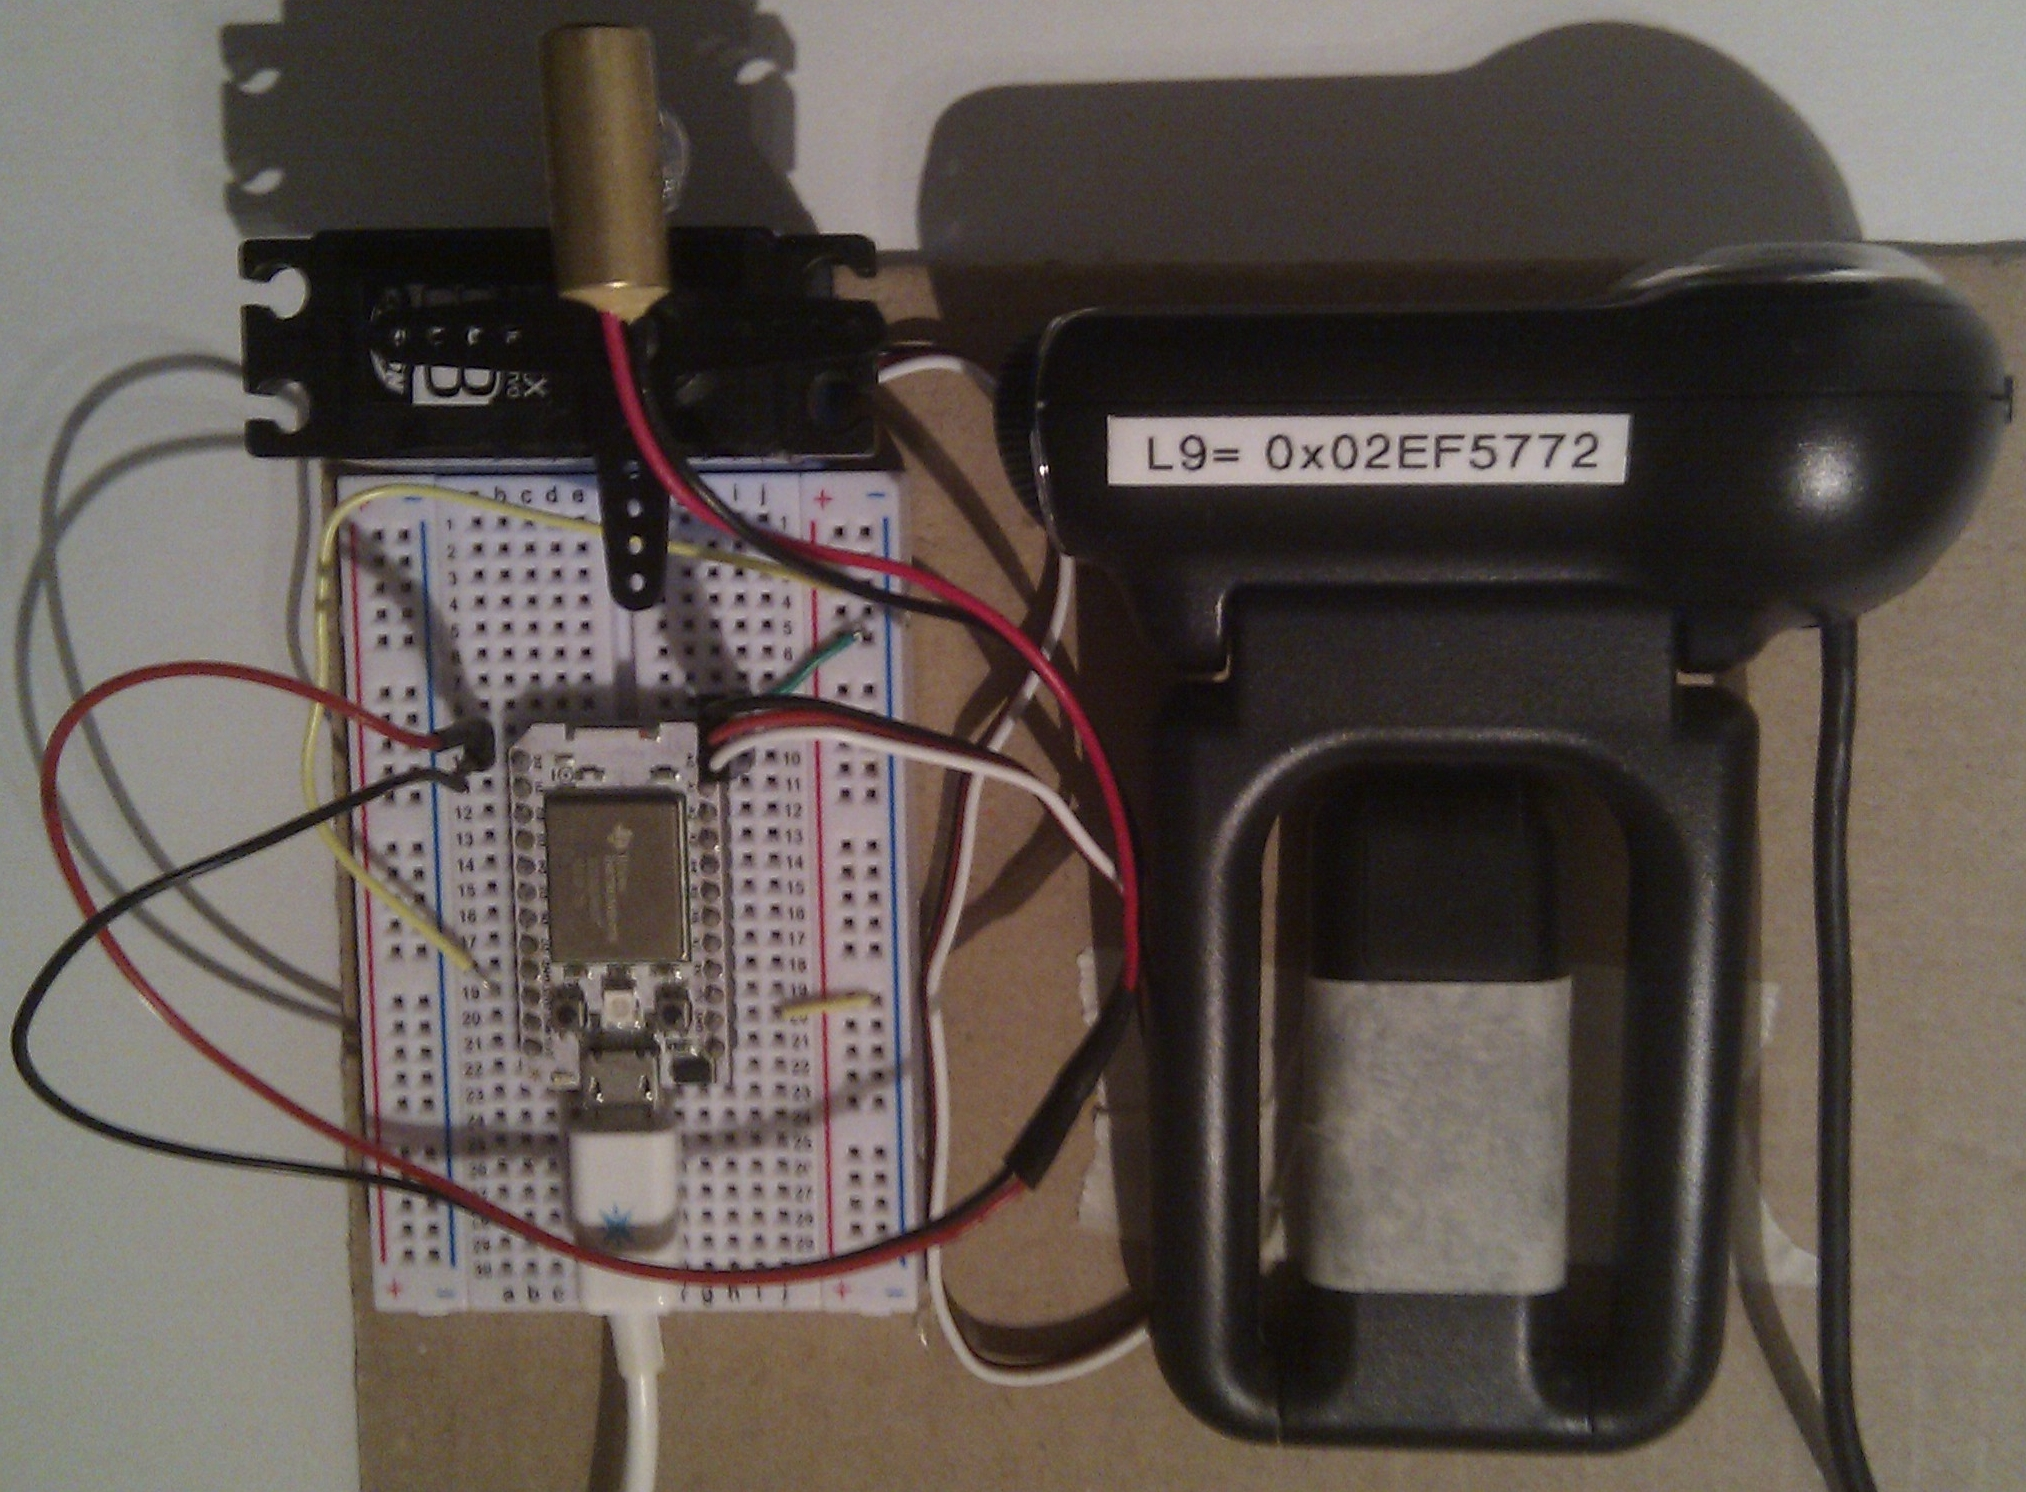
\includegraphics[width=0.9\linewidth]{includes/hardware.jpg}

\end{frame}


%\subsection{Ablauf}
\begin{frame}
	\frametitle{Umsetzung}
	\framesubtitle{Ablauf}

	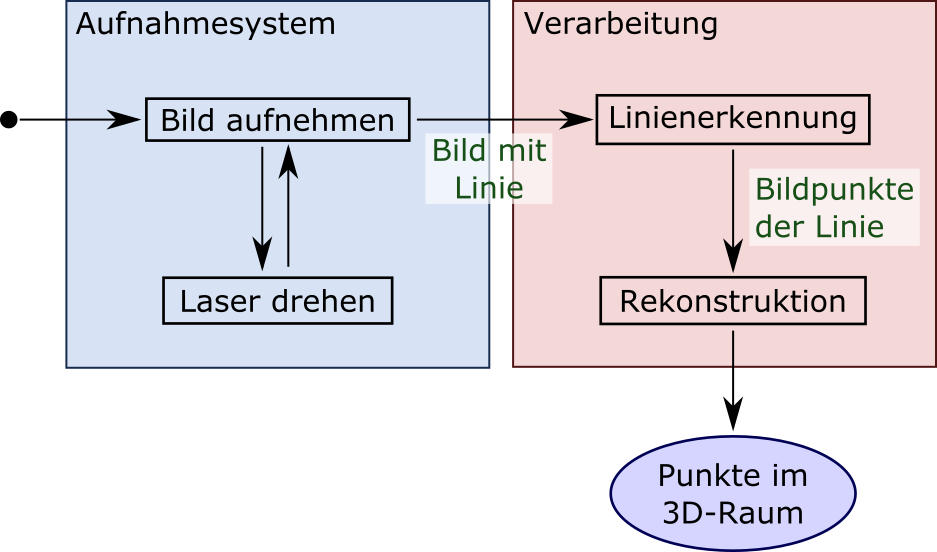
\includegraphics[width=\linewidth]{includes/blockbild.png}

\end{frame}


%\subsection{Linienerkennung}
\begin{frame}
	\frametitle{Umsetzung}
	\framesubtitle{Linienerkennung}

	Einfache Linienerkennung durch Differenzbildung:
	\vfill
	\begin{columns}
		\column{.32\linewidth}{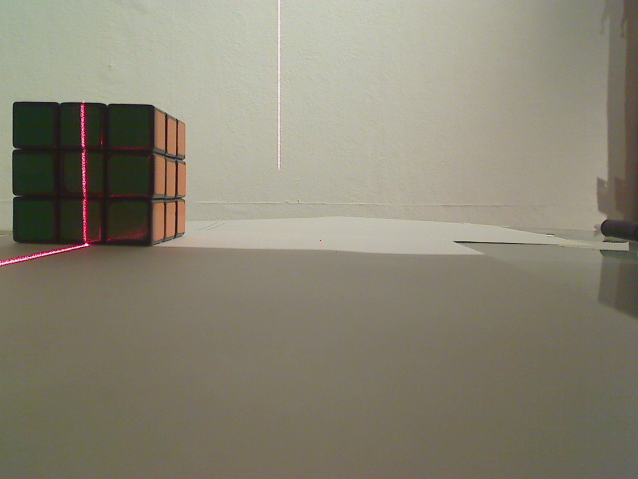
\includegraphics[width=\linewidth]{includes/line_line}}
		\column{.02\linewidth}{$-$}
		\column{.32\linewidth}{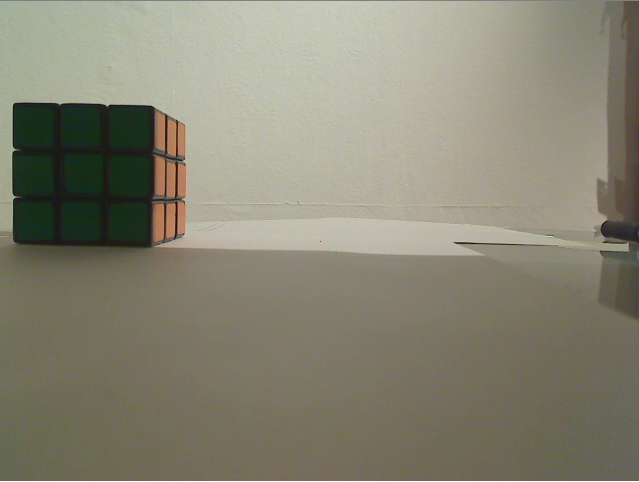
\includegraphics[width=\linewidth]{includes/line_ref}}
		\column{.02\linewidth}{$=$}
		\column{.32\linewidth}{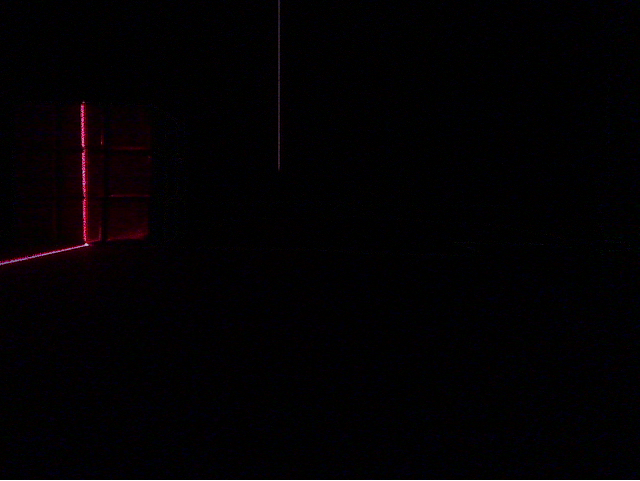
\includegraphics[width=\linewidth]{includes/line_diff}}
	\end{columns}
	\vfill
	\begin{columns}
%		\column{.02\linewidth}{$\Rightarrow$}
		\column{.41\linewidth}{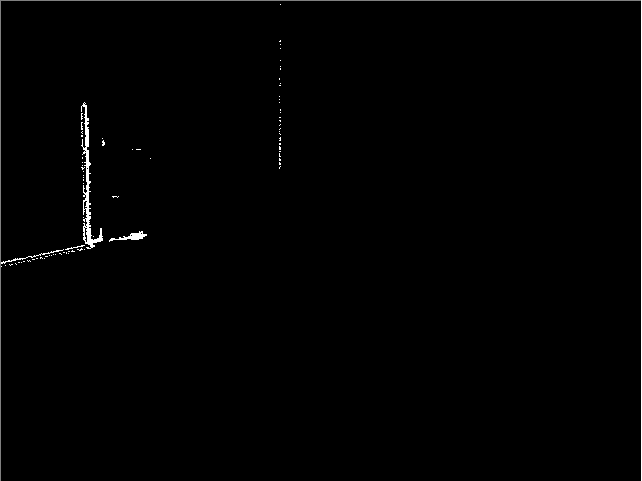
\includegraphics[width=\linewidth]{includes/line_diff_filtered}}
	\end{columns}

\end{frame}


\begin{frame}
	\frametitle{Umsetzung}
	\framesubtitle{Linienerkennung}

	Linienerkennung durch Kanalweise Mittelwertbildung und logische Verknüpfung:\vfill
	\begin{columns}
		\column{.45\linewidth}{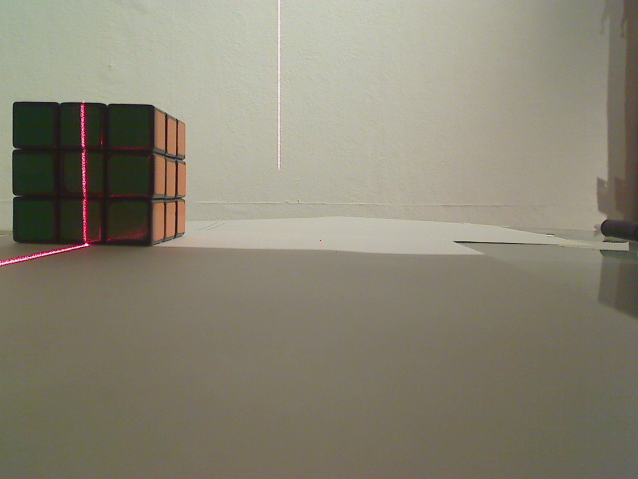
\includegraphics[width=\linewidth]{includes/line_line}}
		\column{.05\linewidth}{$\Rightarrow$}
		\column{.45\linewidth}{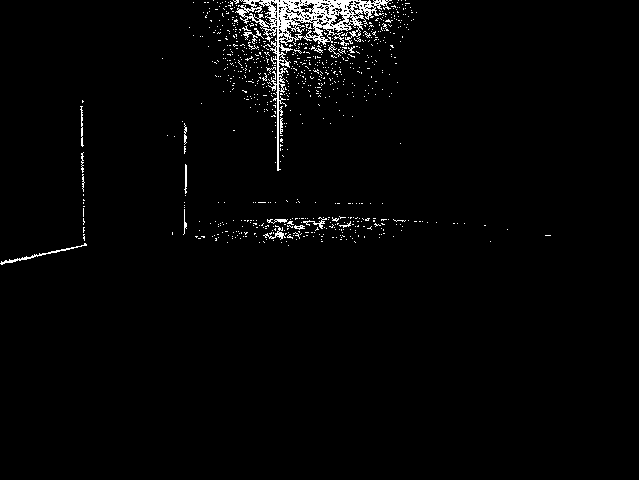
\includegraphics[width=\linewidth]{includes/line_free}}
	\end{columns}

\end{frame}


%\subsection{Rekonstruktion}
\begin{frame}
	\frametitle{Umsetzung}
	\framesubtitle{Rekonstruktion}

	\begin{columns}
		\small
		\begin{column}{.61\linewidth}
			\begin{itemize}
				\item \textbf{Schritt 1:} Berechne die normalisierten Bildkoordinaten $(u,v)$.
				\item \textbf{Schritt 2:} Bestimme $\alpha$, $\beta$, $c$ und $f$ aus der Gerätekonfiguration und den Bildkoordinaten.
				\item \textbf{Schritt 3:} Berechne $h$:
				\[h = \frac{c * \sin(\alpha) * \sin(\beta)}{\sin(180^\circ - \beta - \alpha)}\]
				\item \textbf{Schritt 4:} Bestimme Koordinaten innerhalb der Szene:
				\[\begin{pmatrix}x\\y\\z\end{pmatrix} = \frac{h}{f} *
				\begin{pmatrix}u\\v\\-f\end{pmatrix}\]
			\end{itemize}
		\end{column}
		\begin{column}{.39\linewidth}
			\hfill\fbox{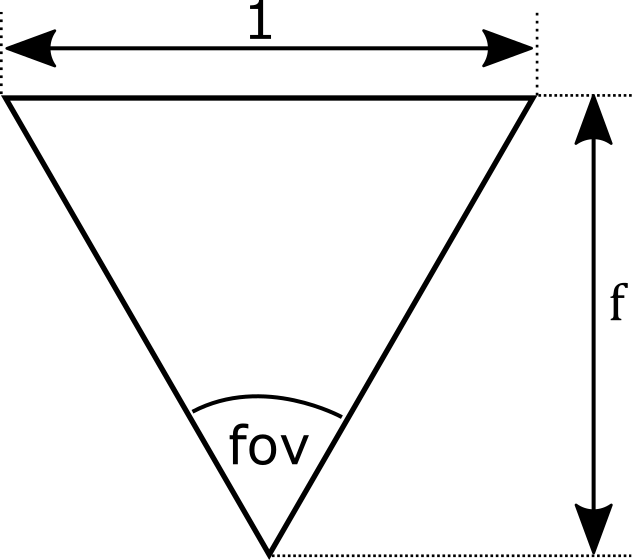
\includegraphics[width=0.9\linewidth]{includes/reconstruction_2}}
			\vfill\vspace{3ex}\vfill
			\hfill\fbox{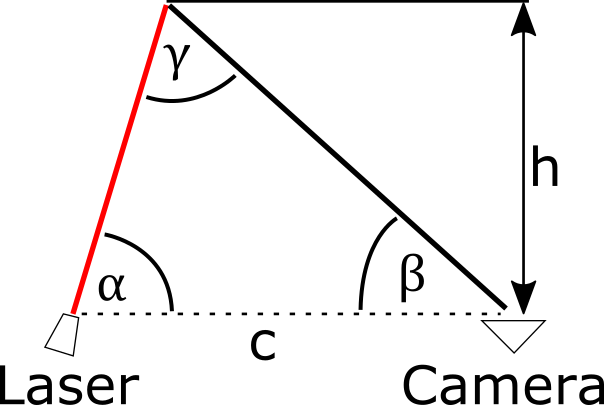
\includegraphics[width=0.9\linewidth]{includes/reconstruction_1}}
		\end{column}
	\end{columns}

\end{frame}


\begin{frame}
	\frametitle{Umsetzung}

	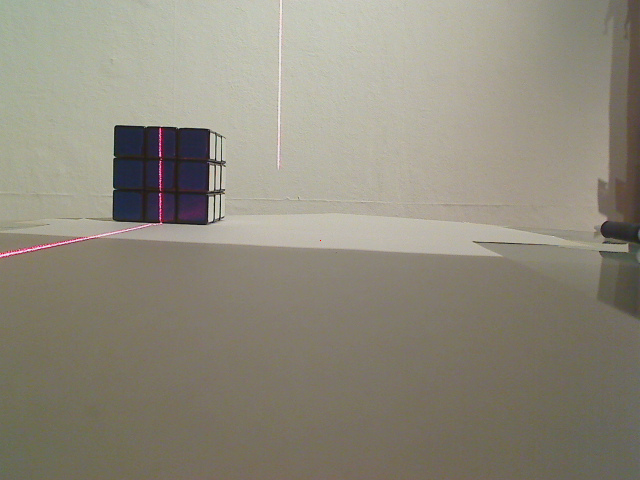
\includegraphics[width=0.9\linewidth]{includes/cap.png}

\end{frame}
\begin{frame}
	\frametitle{Umsetzung}

	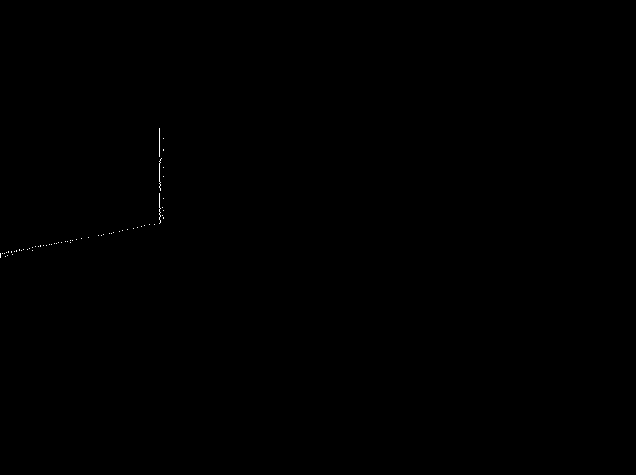
\includegraphics[width=0.9\linewidth]{includes/line.png}

\end{frame}
\begin{frame}
	\frametitle{Umsetzung}

	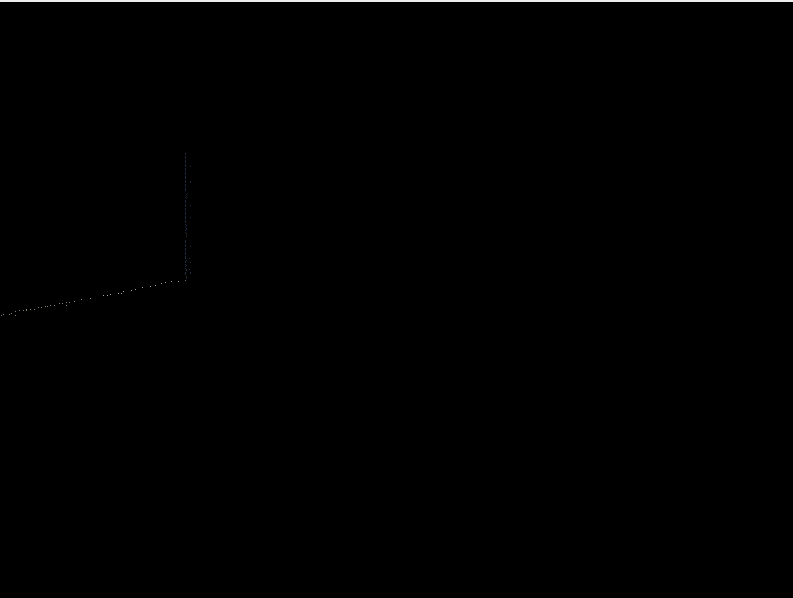
\includegraphics[width=0.9\linewidth]{includes/3d.png}

\end{frame}
\begin{frame}
	\frametitle{Umsetzung}

	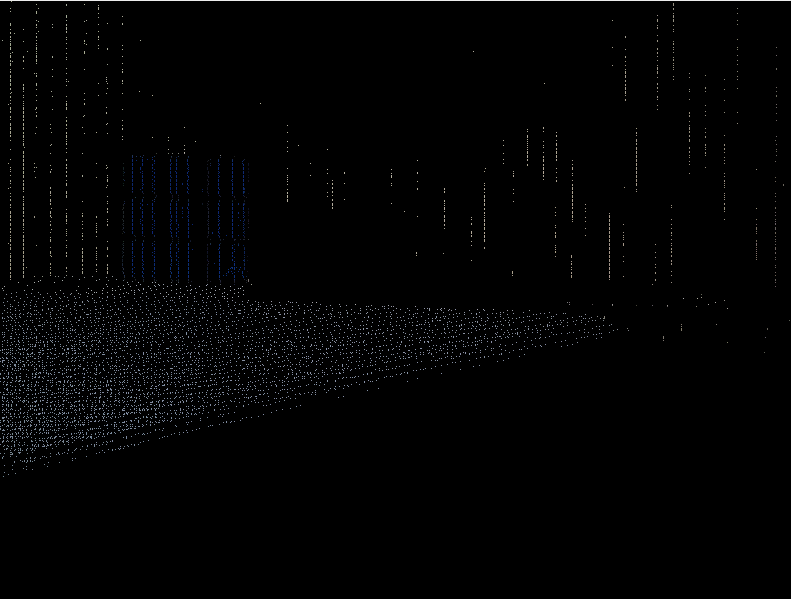
\includegraphics[width=0.9\linewidth]{includes/3d_2.png}

\end{frame}
\begin{frame}
	\frametitle{Umsetzung}

	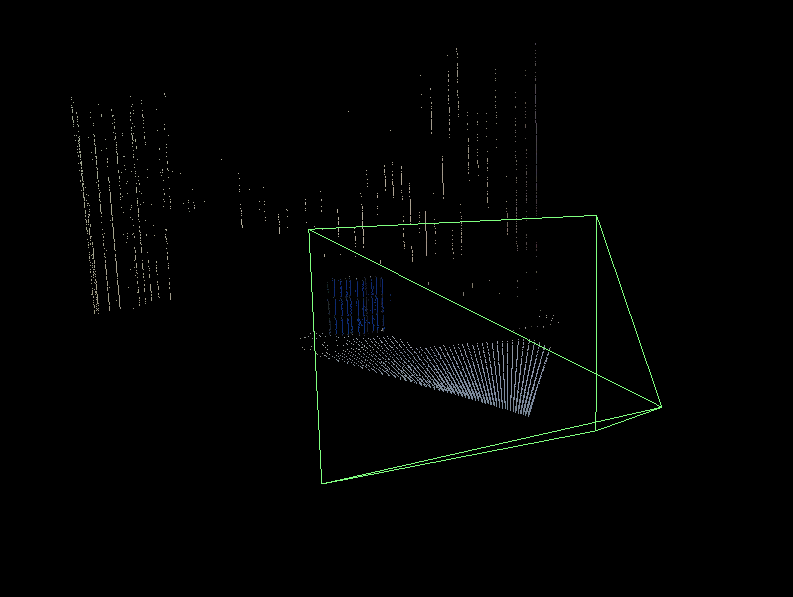
\includegraphics[width=0.9\linewidth]{includes/3d_3.png}

\end{frame}
\begin{frame}
	\frametitle{Umsetzung}

	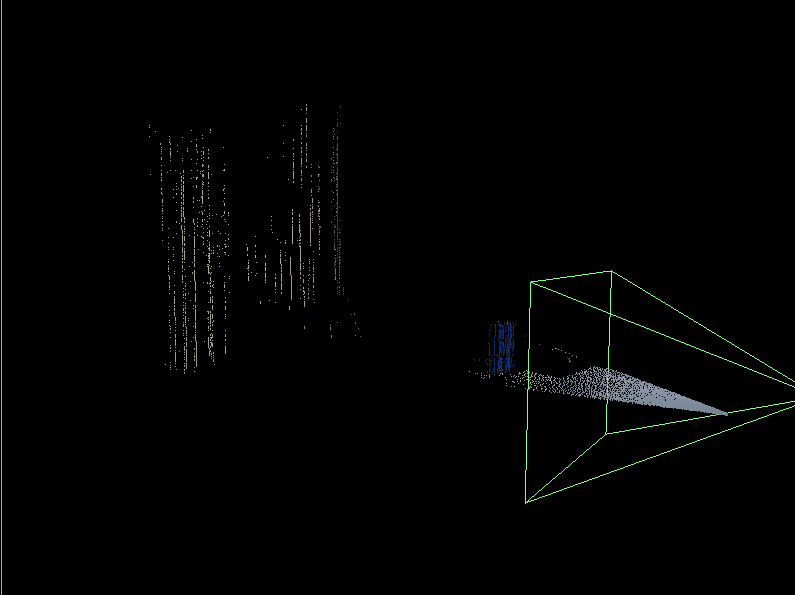
\includegraphics[width=0.9\linewidth]{includes/3d_4.png}

\end{frame}

% ---------------------------------------------------------------------------- %

\section{Probleme}
%\subsection{Organisatorisches}
\begin{frame}
	\frametitle{Probleme}
	\framesubtitle{Organsiatorisches}

	\begin{itemize}
		\item Viel Zeit bei der Planung verloren
		\begin{itemize}
			\item Fehlende Erfahrung bei der Strukturierung solcher Anwendungen
			\item Uneinigkeit bei Schwerpunkten und Verfahren
		\end{itemize}
	\end{itemize}

\end{frame}


%\subsection{Hardware}
\begin{frame}
	\frametitle{Probleme}
	\framesubtitle{Hardware}

	\begin{itemize}
		\item Aufbau der Hardware
		\begin{itemize}
			\item Montage von Laser auf Servo
			\item Montage der Kamera
		\end{itemize}
		\item Ursache für Ungenauigkeiten
		\begin{itemize}
			\item kleine Fehler bei der Montage können u.U. zu großen Fehlern führen
			\item schwer die Winkel und Entfernungen zwischen Kamera, Servo und Laser genau zu messen 
		\end{itemize}
	\end{itemize}

\end{frame}


\begin{frame}
	\frametitle{Probleme}
	\framesubtitle{Hardware}

	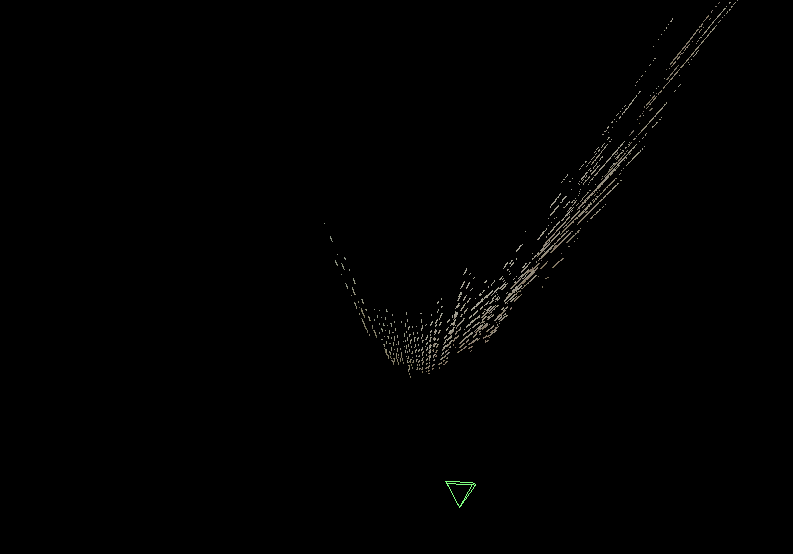
\includegraphics[width=\linewidth]{includes/krumm.png}

\end{frame}


%\subsection{Linienerkennung}
\begin{frame}
	\frametitle{Probleme}
	\framesubtitle{Linienerkennung}

	\begin{itemize}
		\item Hintergrundfarbe
		\item Beleuchtung
	\end{itemize}

\end{frame}

% ---------------------------------------------------------------------------- %

\section{Ergebnisse}
%\subsection{Wiederholte Messungen}
\begin{frame}
	\frametitle{Ergebnisse}
	\framesubtitle{Wiederholte Messungen}

	\begin{figure}
		\begin{minipage}{0.32\linewidth}
			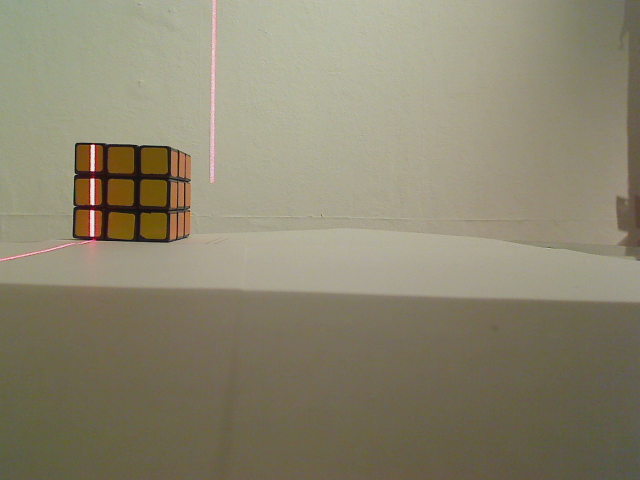
\includegraphics[width=\linewidth]{includes/test_repeat_1}
		\end{minipage}
		\hfill
		\begin{minipage}{0.32\linewidth}
			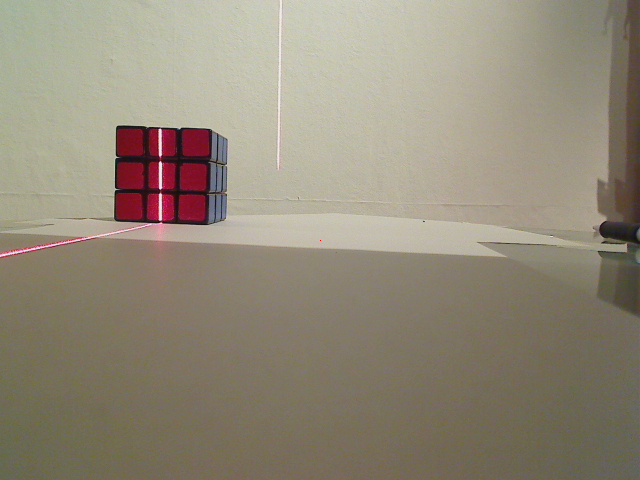
\includegraphics[width=\linewidth]{includes/test_repeat_2}
		\end{minipage}
		\hfill
		\begin{minipage}{0.32\linewidth}
			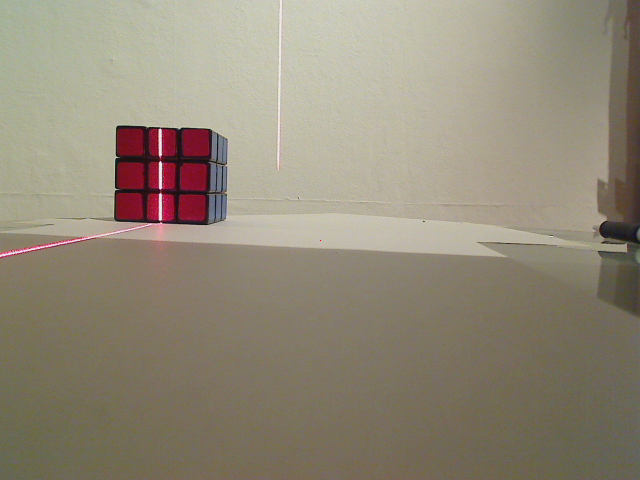
\includegraphics[width=\linewidth]{includes/test_repeat_3}
		\end{minipage}
	\end{figure}
	
	Entfernung: 300mm\\
	Höhe: 56mm\\
	Farbe: Gelb

\end{frame}
	
\begin{frame}
	\frametitle{Ergebnisse}
	\framesubtitle{Wiederholte Messungen}
		\textbf{Entfernung}\\
	
		Linienerkennung mit Differenzbild
		\begin{tabular}{c|c|c|c|c|c}
			Messung & Min & Max & Avg & Diff (\%) & Stdabw \\ \hline
1 & 298.3 & 21629.5 & 348.7 & 16.2 & 909.1 \\
2 & 287.1 & 327.1 & 309.1 & 3.0 & 5.1 \\
3 & 287.1 & 327.1 & 309.9 & 3.3 & 6.0 \\
4 & 287.1 & 327.1 & 310.1 & 3.4 & 5.5 \\
5 & 287.1 & 458.0 & 310.2 & 3.4 & 7.3 \\
6 & 287.1 & 335.8 & 310.5 & 3.5 & 5.4 \\
7 & 299.8 & 15381.7 & 342.8 & 14.3 & 645.7 \\
8 & 299.0 & 327.1 & 309.4 & 3.1 & 5.0 \\
9 & 293.5 & 327.1 & 309.7 & 3.2 & 5.3 \\
10 & 287.1 & 11934.4 & 320.8 & 6.9 & 355.1
		\end{tabular}
		
\end{frame}
	
\begin{frame}
	\frametitle{Ergebnisse}
	\framesubtitle{Wiederholte Messungen}
		\textbf{Entfernung}\\
	
		Linienerkennung ohne Differenzbild
		\begin{tabular}{c|c|c|c|c|c}
			Messung & Min & Max & Avg & Diff (\%) & Stdabw \\ \hline
1 & 300.7 & 325.1 & 307.6 & 2.5 & 4.3\\
2 & 77.0 & 323.1 & 243.1 & -19.0 & 101.2\\
3 & 300.7 & 325.1 & 307.9 & 2.6 & 4.3\\
4 & 77.0 & 327.1 & 250.7 & -16.4 & 97.4\\
5 & 300.7 & 327.1 & 307.9 & 2.6 & 4.1\\
6 & 77.0 & 327.1 & 246.4 & -17.9 & 99.7\\
7 & 300.7 & 323.1 & 307.5 & 2.5 & 3.8\\
8 & 300.7 & 327.1 & 308.1 & 2.7 & 4.3\\
9 & 77.0 & 323.1 & 251.1 & -16.3 & 97.3\\
10 & 80.2 & 325.1 & 278.0 & -7.3 & 75.6
		\end{tabular}
	
\end{frame}

\begin{frame}
	\frametitle{Ergebnisse}
	\framesubtitle{Wiederholte Messungen}
		\textbf{Höhe}\\
		
		Linienerkennung mit Differenzbild
		\begin{tabular}{c|c|c}
			Messung & Hoehe & Diff (\%) \\ \hline
1 & 48.6 & -13.2 \\
2 & 34.4 & -38.7 \\
3 & 27.8 & -50.3 \\
4 & 28.6 & -48.9 \\
5 & 49.2 & -12.2 \\
6 & 32.6 & -41.8 \\
7 & 27.2 & -51.3 \\
8 & 27.2 & -51.3 \\
9 & 34.4 & -38.7 \\
10 & 48.0 & -14.3\\

		\end{tabular}
		
		
\end{frame}

\begin{frame}
	\frametitle{Ergebnisse}
	\framesubtitle{Wiederholte Messungen}
		\textbf{Höhe}\\
		
		Linienerkennung ohne Differenzbild
		\begin{tabular}{c|c|c|c|c|c}
			Messung & Hoehe & Diff (\%) \\ \hline
1 & 54.8 &  -2.2 \\
2 & 54.4 &  -2.9 \\
3 & 54.7 &  -2.3 \\
4 & 54.7 &  -2.3 \\
5 & 54.7 &  -2.3 \\
6 & 53.2 &  -4.9 \\
7 & 53.9 &  -3.8 \\
8 & 53.5 &  -4.4 \\
9 & 53.5 &  -4.4 \\
10 & 53.5 & -4.4 \\


		\end{tabular}
		
\end{frame}

%\subsection{Verschiedene Farben}
\begin{frame}
	\frametitle{Ergebnisse}
	\framesubtitle{Verschiedene Farben}

	\begin{figure}
		\begin{minipage}{0.32\linewidth}
			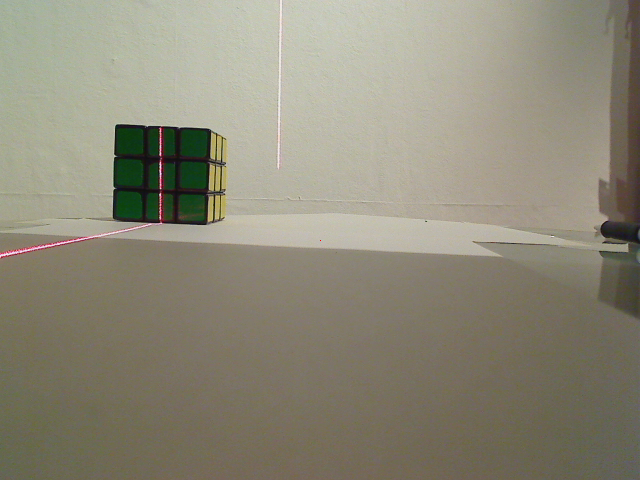
\includegraphics[width=\linewidth]{includes/test_color_1}
		\end{minipage}
		\hfill
		\begin{minipage}{0.32\linewidth}
			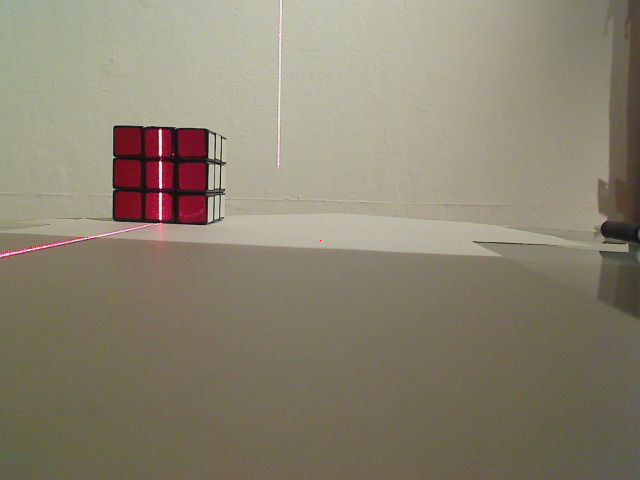
\includegraphics[width=\linewidth]{includes/test_color_2}
		\end{minipage}
		\hfill
		\begin{minipage}{0.32\linewidth}
			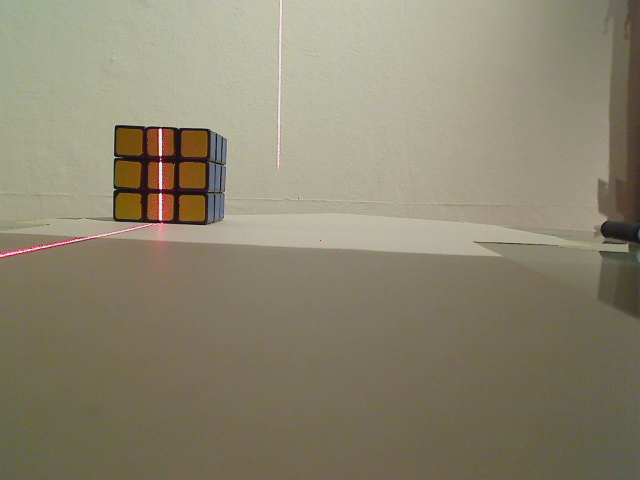
\includegraphics[width=\linewidth]{includes/test_color_3}
		\end{minipage}
	\end{figure}
	
	Entfernung: 300mm\\
	Höhe: 56mm\\
	Verschiedene Farben\\
	je 10 Messungen
	
\end{frame}
	
\begin{frame}
	\frametitle{Ergebnisse}
	\framesubtitle{Verschiedene Farben}
		\textbf{Entfernung}\\
		
		Linienerkennung mit Differenzbild
		\begin{tabular}{c|c|c|c|c|c}
			Farbe & Min & Max & Avg & Diff (\%) & Stdabw\\ \hline
Blau &-1.3 & 351.5 & 309.0 & 3.0 & 10.8\\
Grün &-1.3 & 36424.6 & 353.8 & 17.9 & 1054.2\\
Orange &-1.3 & 21629.5 & 313.3 & 4.4 & 274.3\\
Rot &-1.3 & 36424.6 & 331.0 & 10.3 & 789.8\\
Gelb &-1.3 & 21629.5 & 318.3 & 6.1 & 379.5\\
		\end{tabular}
		
\end{frame}

\begin{frame}
	\frametitle{Ergebnisse}
	\framesubtitle{Verschiedene Farben}
		\textbf{Entfernung}\\
		
		Linienerkennung ohne Differenzbild
		\begin{tabular}{c|c|c|c|c|c}
			Farbe & Min & Max & Avg & Diff (\%) & Stdabw\\ \hline
Blau &-1.3 & 325.1 & 310.7 & 3.6 & 18.3\\
Grün &-1.3 & 325.1 & 301.2 & 0.4 & 47.8\\
Orange &-1.3 & 15381.7 & 309.8 & 3.3 & 186.2\\
Rot &-1.3 & 329.1 & 306.2 & 2.1 & 21.6\\
Gelb & -1.3 & 327.1 & 276.5 & -7.8 & 77.8\\
		\end{tabular}

\end{frame}


\begin{frame}
	\frametitle{Ergebnisse}
	\framesubtitle{Verschiedene Farben}
		\textbf{Höhe}\\
		
		Linienerkennung mit Differenzbild
		\begin{tabular}{c|c|c|c|c|c}
			Farbe & Min & Max & Avg & Diff (\%) & Stdabw\\ \hline
Blau &   54.3 & 56.4 & 55.5 & -0.8 & 0.8\\
Grün &    39.9 & 98.4 & 58.1 & 3.8 & 14.2\\
Orange&     32.0 & 56.1 & 45.4 & -19.0 & 7.3\\
Rot &    29.8 & 69.9 & 41.5 & -25.9 & 11.3\\
Gelb &     27.2 & 49.2 & 35.8 & -36.1 & 8.8\\

		\end{tabular}
		
		
\end{frame}

\begin{frame}
	\frametitle{Ergebnisse}
	\framesubtitle{Verschiedene Farben}
		\textbf{Höhe}\\
		
		Linienerkennung ohne Differenzbild
		\begin{tabular}{c|c|c|c|c|c}
			Farbe & Min & Max & Avg & Diff (\%) & Stdabw\\ \hline
Blau &    52.1 & 55.1 & 53.8 & -3.9 & 1.0\\
Grün &     54.2 & 55.7 & 54.9 & -2.0 & 0.4\\
Orange&     54.5 & 55.4 & 54.6 & -2.4 & 0.3\\
Rot &    54.7 & 56.1 & 55.2 & -1.4 & 0.3\\
Gelb &      53.2 & 54.8 & 54.1 & -3.4 & 0.6\\

		\end{tabular}
		
		
\end{frame}


%\subsection{Verschiedene Entfernungen}
\begin{frame}
	\frametitle{Ergebnisse}
	\framesubtitle{Verschiedene Entfernungen}

	\begin{figure}
		\begin{minipage}{0.32\linewidth}
			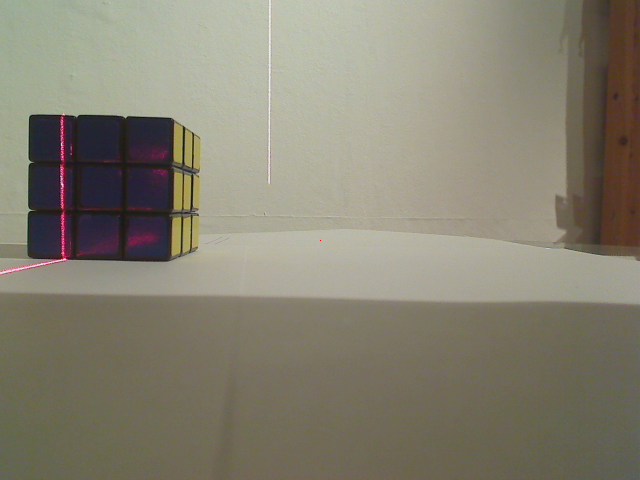
\includegraphics[width=\linewidth]{includes/test_dist_1}
		\end{minipage}
		\hfill
		\begin{minipage}{0.32\linewidth}
			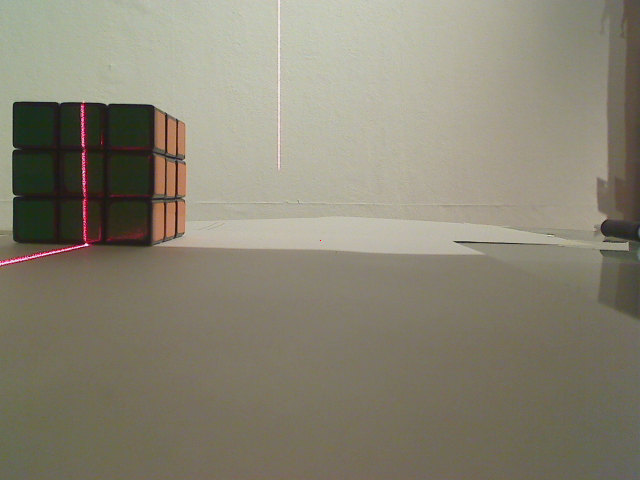
\includegraphics[width=\linewidth]{includes/test_dist_2}
		\end{minipage}
		\hfill
		\begin{minipage}{0.32\linewidth}
			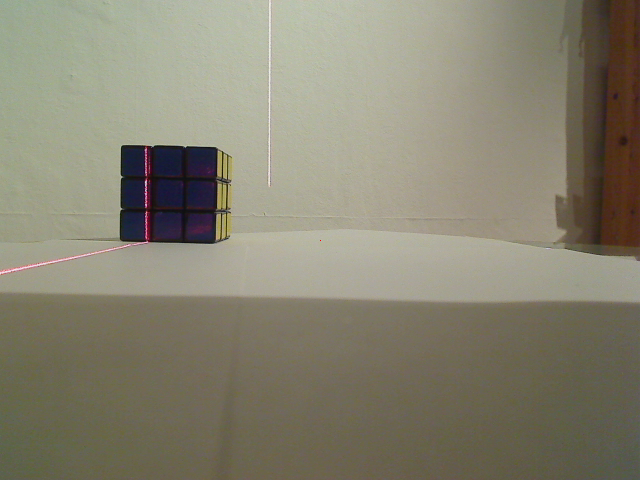
\includegraphics[width=\linewidth]{includes/test_dist_3}
		\end{minipage}
	\end{figure}
	Verschiedene Entfernungen\\
	Höhe: 56mm\\
	Farbe: Blau\\
	je 10 Messungen
	
\end{frame}

\begin{frame}
	\frametitle{Ergebnisse}
	\framesubtitle{Verschiedene Entfernungen}
		\textbf{Entfernung}\\
		
		Linienerkennung mit Differenzbild
		\begin{tabular}{c|c|c|c|c|c}
			Entfernung & Min & Max & Avg & Diff (\%) & Stdabw\\ \hline
150 &      -1.3 & 477.4 & 172.6 & -42.5 & 34.7\\
200 &      -1.3 & 392.0 & 215.4 & -28.2 & 23.3\\
250 &      -1.3 & 864.4 & 261.8 & -12.7 & 15.6\\
300 &      -1.3 & 351.5 & 309.0 & 3.0 & 10.8\\

		\end{tabular}
		
		
\end{frame}

\begin{frame}
	\frametitle{Ergebnisse}
	\framesubtitle{Verschiedene Entfernungen}
		\textbf{Entfernung}\\
		
		Linienerkennung ohne Differenzbild
		\begin{tabular}{c|c|c|c|c|c}
			Entfernung & Min & Max & Avg & Diff (\%) & Stdabw\\ \hline
150 &      -1.3 & 398.8 & 146.6 & -51.1 & 48.3\\
200 &      -1.3 & 375.2 & 210.9 & -29.7 & 31.5\\
250 &      -1.3 & 375.2 & 261.0 & -13.0 & 21.9\\
300 &   -1.3 & 325.1 & 310.7 & 3.6 & 18.3\\
		\end{tabular}

\end{frame}



\begin{frame}
	\frametitle{Ergebnisse}
	\framesubtitle{Verschiedene Entfernungen}
		\textbf{Höhe}\\
		
		Linienerkennung mit Differenzbild
		\begin{tabular}{c|c|c|c|c|c}
			Entfernung & Min & Max & Avg & Diff (\%) & Stdabw\\ \hline
150 &     39.1 & 56.6 & 50.7 & -9.5 & 4.2\\
200 &     42.4 & 57.3 & 54.0 & -3.6 & 5.1\\
250 &     43.6 & 56.8 & 51.7 & -7.6 & 5.1\\
300 &  54.3 & 56.4 & 55.5 & -0.8 & 0.8\\


		\end{tabular}
\end{frame}


\begin{frame}
	\frametitle{Ergebnisse}
	\framesubtitle{Verschiedene Entfernungen}
		\textbf{Höhe}\\
		
		Linienerkennung ohne Differenzbild
		\begin{tabular}{c|c|c|c|c|c}
			Entfernung & Min & Max & Avg & Diff (\%) & Stdabw\\ \hline
150 &     21.9 & 56.7 & 36.0 & -35.6 & 12.6\\
200 &     54.9 & 56.5 & 55.8 & -0.4 & 0.5\\
250 &     54.4 & 55.9 & 54.9 & -1.9 & 0.4\\
300 &     52.1 & 55.1 & 53.8 & -3.9 & 1.0\\

		\end{tabular}
\end{frame}

% ---------------------------------------------------------------------------- %

\section{Zusammenfassung und Ausblick}
\begin{frame}
	\frametitle{Zusammenfassung}

	\begin{itemize}
		\item Grobe Vermessung funktioniert
		\item Defizite bei der Genauigkeit durch ungenaue und/oder mangelhaft kalibrierte Hardware
	\end{itemize}

\end{frame}


\begin{frame}
	\frametitle{Ausblick}

	\begin{itemize}
		\item Fehler durch bessere Kalibrierung und/oder besseres Setup minimieren
		\item Linienerkennung (ohne Referenzbild) robuster gestalten
		\item Objekt statt Laser bewegen
	\end{itemize}

\end{frame}

% ---------------------------------------------------------------------------- %

\section{Live-Demo} 
\begin{frame}
	\frametitle{Live-Demo}
\end{frame}

% ---------------------------------------------------------------------------- %

\section{Quellen} 
\begin{frame}
	\frametitle{Quellen}

\end{frame}


\end{document}
